\documentclass{beamer}\usepackage[]{graphicx}\usepackage[]{color}
%% maxwidth is the original width if it is less than linewidth
%% otherwise use linewidth (to make sure the graphics do not exceed the margin)
\makeatletter
\def\maxwidth{ %
  \ifdim\Gin@nat@width>\linewidth
    \linewidth
  \else
    \Gin@nat@width
  \fi
}
\makeatother

\definecolor{fgcolor}{rgb}{0.345, 0.345, 0.345}
\newcommand{\hlnum}[1]{\textcolor[rgb]{0.686,0.059,0.569}{#1}}%
\newcommand{\hlstr}[1]{\textcolor[rgb]{0.192,0.494,0.8}{#1}}%
\newcommand{\hlcom}[1]{\textcolor[rgb]{0.678,0.584,0.686}{\textit{#1}}}%
\newcommand{\hlopt}[1]{\textcolor[rgb]{0,0,0}{#1}}%
\newcommand{\hlstd}[1]{\textcolor[rgb]{0.345,0.345,0.345}{#1}}%
\newcommand{\hlkwa}[1]{\textcolor[rgb]{0.161,0.373,0.58}{\textbf{#1}}}%
\newcommand{\hlkwb}[1]{\textcolor[rgb]{0.69,0.353,0.396}{#1}}%
\newcommand{\hlkwc}[1]{\textcolor[rgb]{0.333,0.667,0.333}{#1}}%
\newcommand{\hlkwd}[1]{\textcolor[rgb]{0.737,0.353,0.396}{\textbf{#1}}}%
\let\hlipl\hlkwb

\usepackage{framed}
\makeatletter
\newenvironment{kframe}{%
 \def\at@end@of@kframe{}%
 \ifinner\ifhmode%
  \def\at@end@of@kframe{\end{minipage}}%
  \begin{minipage}{\columnwidth}%
 \fi\fi%
 \def\FrameCommand##1{\hskip\@totalleftmargin \hskip-\fboxsep
 \colorbox{shadecolor}{##1}\hskip-\fboxsep
     % There is no \\@totalrightmargin, so:
     \hskip-\linewidth \hskip-\@totalleftmargin \hskip\columnwidth}%
 \MakeFramed {\advance\hsize-\width
   \@totalleftmargin\z@ \linewidth\hsize
   \@setminipage}}%
 {\par\unskip\endMakeFramed%
 \at@end@of@kframe}
\makeatother

\definecolor{shadecolor}{rgb}{.97, .97, .97}
\definecolor{messagecolor}{rgb}{0, 0, 0}
\definecolor{warningcolor}{rgb}{1, 0, 1}
\definecolor{errorcolor}{rgb}{1, 0, 0}
\newenvironment{knitrout}{}{} % an empty environment to be redefined in TeX

\usepackage{alltt}
%\usetheme{metropolis}
\usepackage[utf8]{inputenc}
\usepackage{amsfonts}
\usepackage{amsmath}
\usepackage{natbib}
\usepackage{graphicx}
\usepackage{array,booktabs,tabularx}
\usepackage{epstopdf}
\usepackage{colortbl, xcolor}
\usepackage{url}

\newcommand\Fontvi{\fontsize{6}{7.2}\selectfont}

\title{Przewidywanie właściwości sekwencji biologicznych w oparciu o analizę n-gramów}
\date{}
\author{Michał Burdukiewicz}
\institute{Zakład Genomiki i Bioinformatyki, Uniwersytet Wrocławski}
\IfFileExists{upquote.sty}{\usepackage{upquote}}{}
\begin{document}


  

\maketitle

\begin{frame}{Outline}

\tableofcontents

\end{frame} 

\begin{frame}{} 

\textit{In silico} research allows scientists to more efficiently design experimental studies.

Examples: 

\begin{itemize}
\item prediction of protein properties (presence of signal peptides, amyloidogenicity),  
\item predicting culture conditions of bacteria.
\end{itemize}

\end{frame}   
  
\begin{frame}{Aim} 

Create efficient methods for analysis of biological sequences that have human-readable decision rules.

\end{frame}   


\begin{frame}{Amyloid proteins}

Amyloid are proteins associated with various diseases (e.g., Alzheimer’s,
Creutzfeldt-Jakob’s and Huntington’s diseases) which are able to form harmful aggregates.

\begin{figure} 
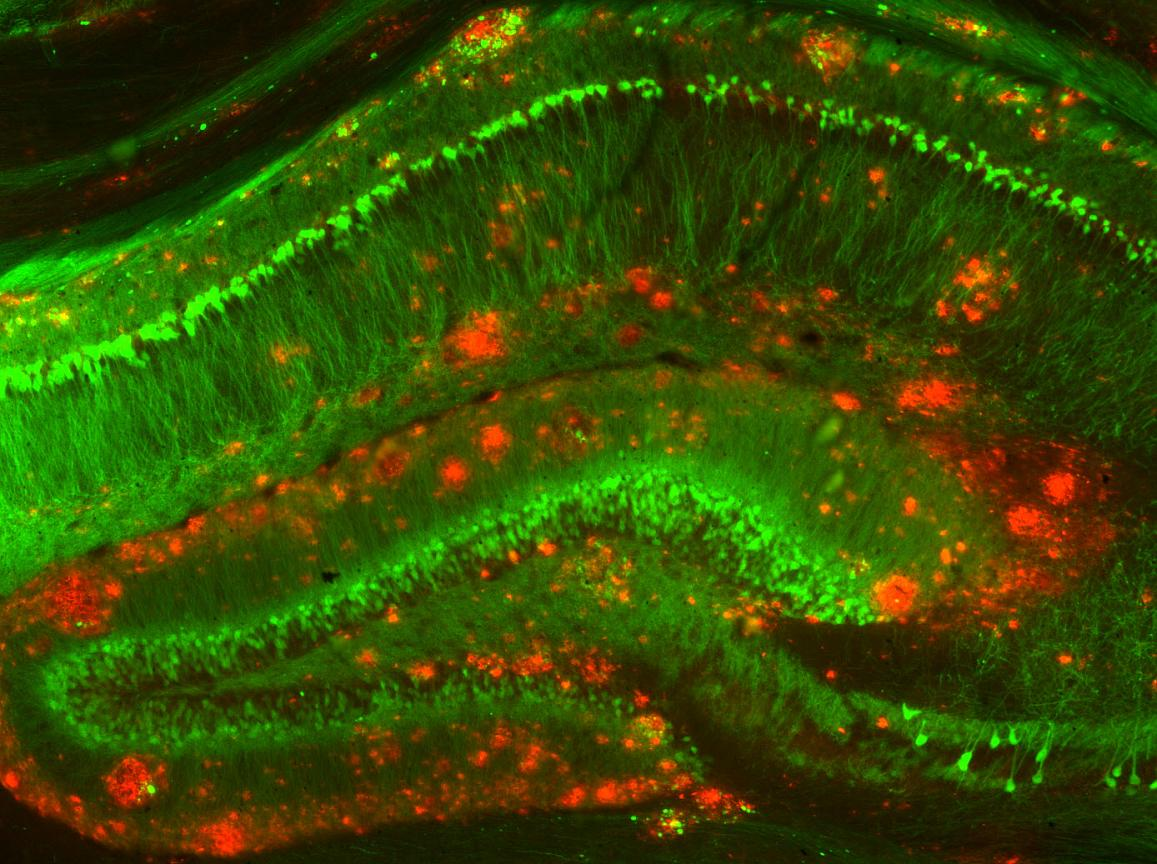
\includegraphics[width=0.61\textwidth]{static_figure/amyloid_aggregates.jpg}
\end{figure}

\footnotesize
Amyloid aggregates (red) around neurons (green). Strittmatter Laboratory, Yale University.

\end{frame}  

  
\begin{frame}{Amyloid proteins}

Hot-spots:
\begin{itemize}
\item short (6-15 amino acids),
\item very high variability of amino acid composition,
\item initiate amyloid aggregation,
\item create specific "zipper-like" $\beta$-structures.
\end{itemize}

\begin{figure} 
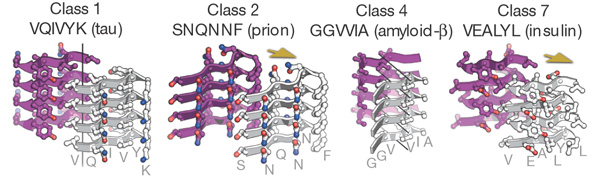
\includegraphics[width=0.9\textwidth]{static_figure/zipper_structure.jpg}
\end{figure}

\footnotesize\citet{sawaya_atomic_2007}
\end{frame}
  
\begin{frame}{Signal peptides}

\begin{figure} 
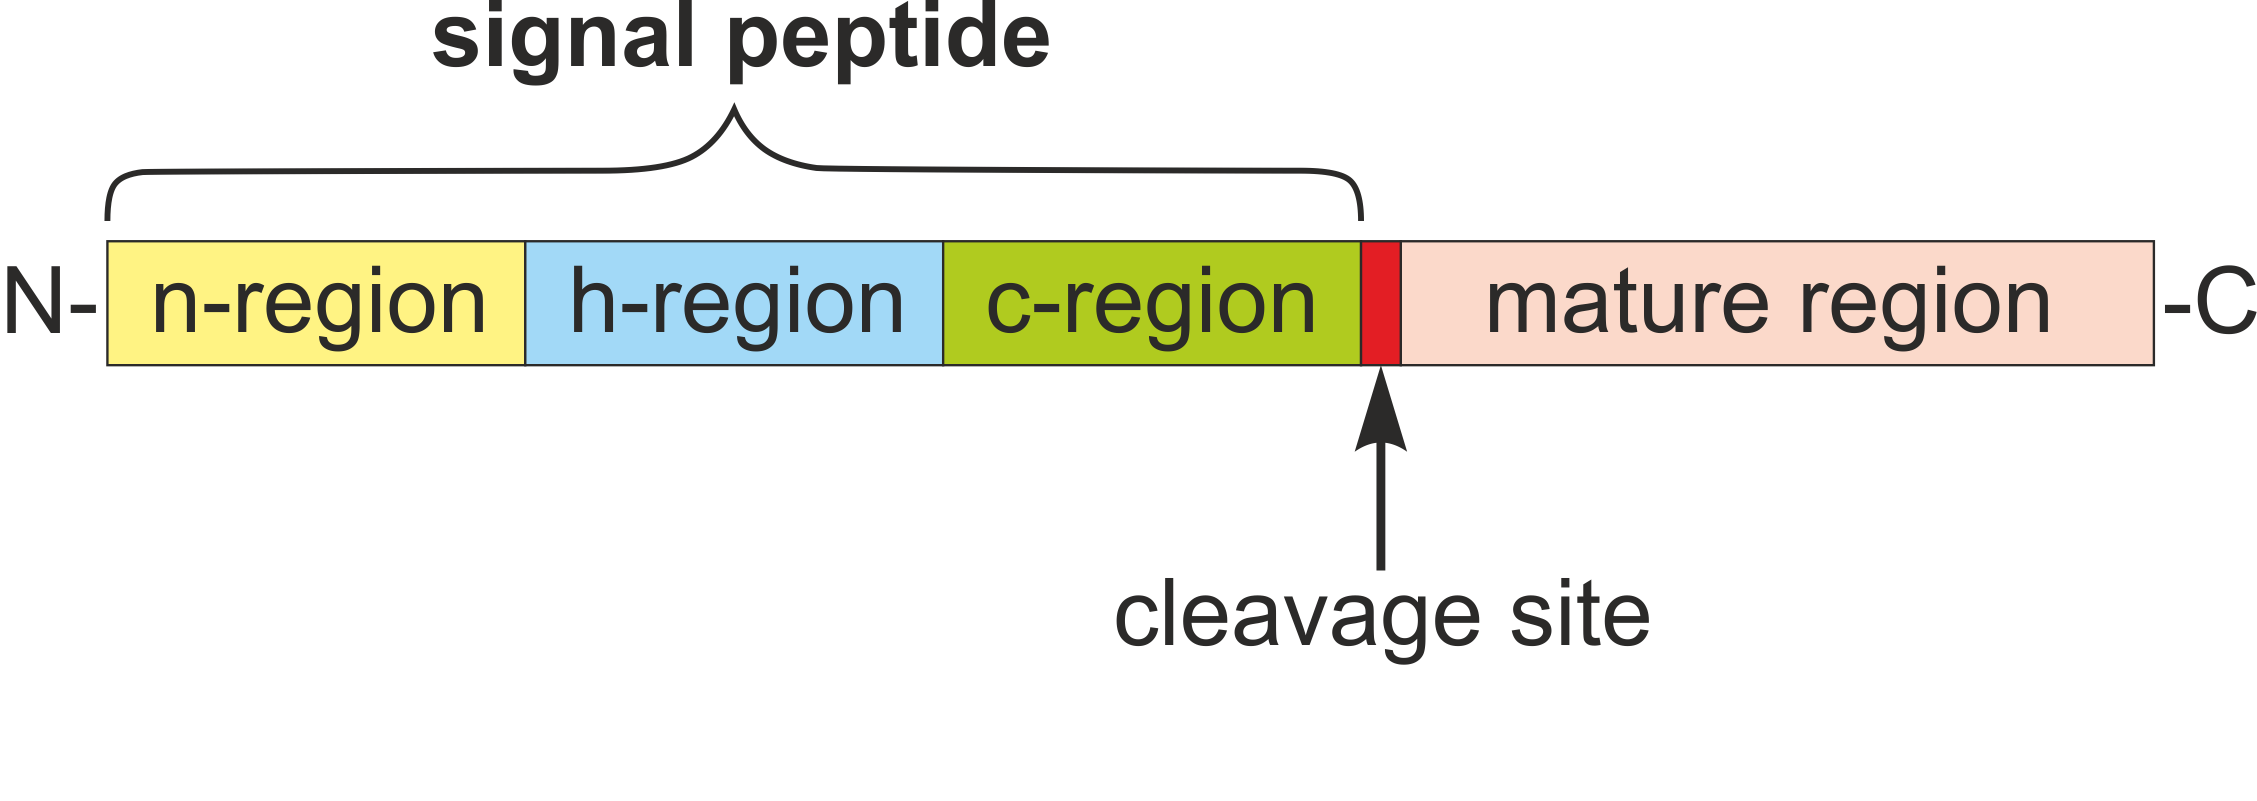
\includegraphics[width=0.75\textwidth]{static_figure/SP.png}
\end{figure}

Signal peptides:
        \begin{itemize}[<+->]
          \item are short (20-30 residues) N-terminal amino acid sequences forming $\alpha$-helices,
            \item direct proteins to the endomembrane system and next to extra- or intracellular localizations,
            \item are universal enough to direct properly proteins in different secretory systems.
        \end{itemize}
\end{frame}


  
\begin{frame}{Signal peptides}

\begin{figure} 
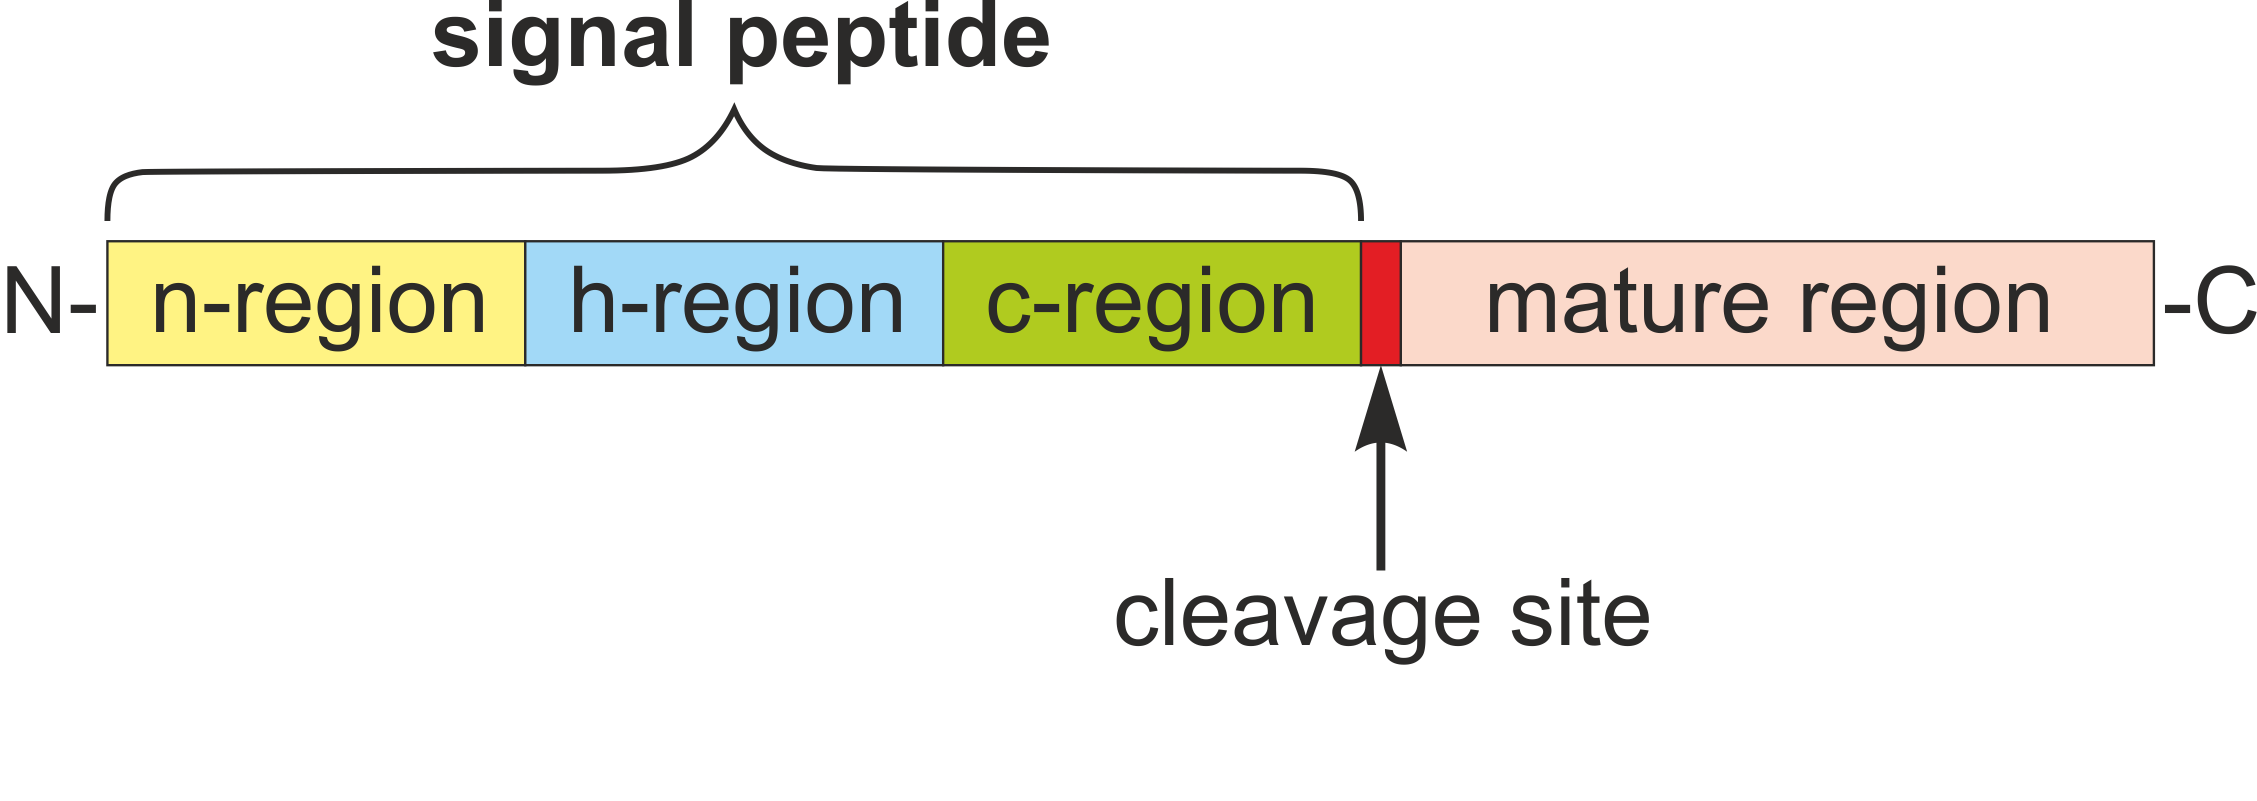
\includegraphics[width=0.75\textwidth]{static_figure/SP.png}
\end{figure}

Signal peptides possess three distinct domains with variable length and characteristic amino acid composition~\citep{hegde_surprising_2006}:
      \begin{itemize}
        \item n-region: mostly basic residues~\citep{nielsen_prediction_1998},
        \item h-region: strongly hydrophobic residues~\citep{nielsen_prediction_1998},
        \item c-region: a few polar, uncharged residues.
      \end{itemize}
\end{frame}


%Peptydy sygnałowe rozpoczynają się naładowanym dodatnio n-regionem, po którym występuje hydrofobowy h-region i c-region zakończony miejscem cięcia rozpoznawanym przez peptydazę sygnałową. 

  
\begin{frame}{Signal peptides}  
Amino acid composition of signal peptides differ between Plasmodium sp. and other eukaryotes. Therefore, predictors of signal peptides do not detect malarial signal peptides accurately.


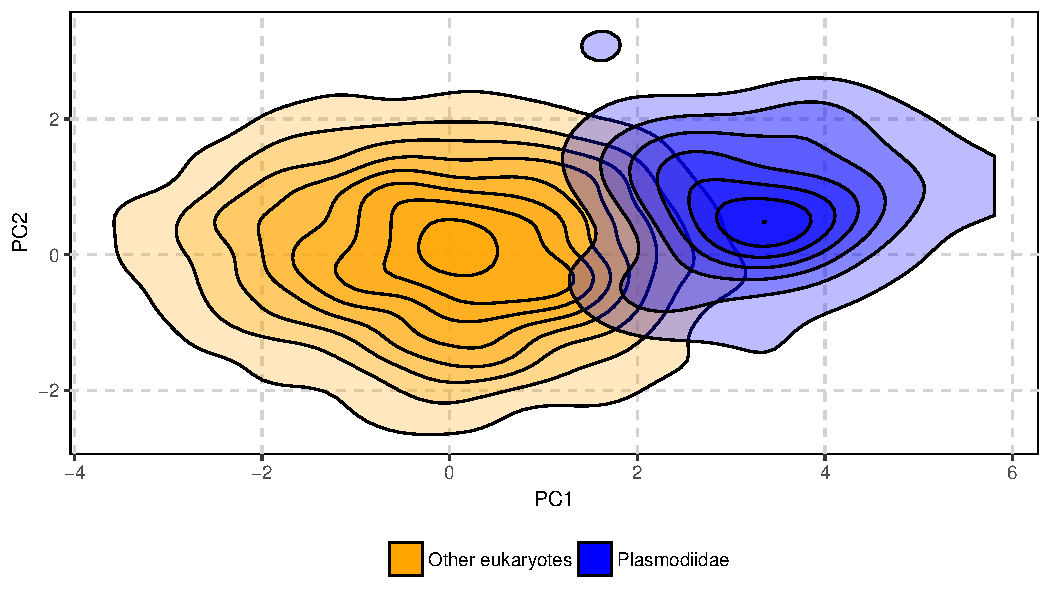
\includegraphics[width=\maxwidth]{figure/unnamed-chunk-1-1} 


PCA of amino acid frequency in signal peptides.
\end{frame}  

\section{n-grams}

\begin{frame}
Computational analysis of biological sequences requires converting them to features understandable by machines.

The optimal conversion of information:
\begin{itemize}
\item loss-less,
\item concise.
\end{itemize}
\end{frame}  

\begin{frame}
n-grams (k-tuples, k-mers):
\begin{itemize}
\item subsequences (continuous or gapped) of $n$ residues,
\item considers the context of a specific residue.
\end{itemize}


% latex table generated in R 3.5.1 by xtable 1.8-3 package
% Tue Nov 20 12:50:40 2018
\begin{table}[ht]
\centering
\begin{tabular}{rlllll}
  \hline
 & P1 & P2 & P3 & P4 & P5 \\ 
  \hline
S1 & M & R & K & L & Y \\ 
   \hline
\end{tabular}
\end{table}



2-grams:
MR, RK, KL, LY

2-grams (gap 1):
M -- K, R -- L, K -- Y

3-grams:
MRK, RKL, KLY
\end{frame}  



\begin{frame}

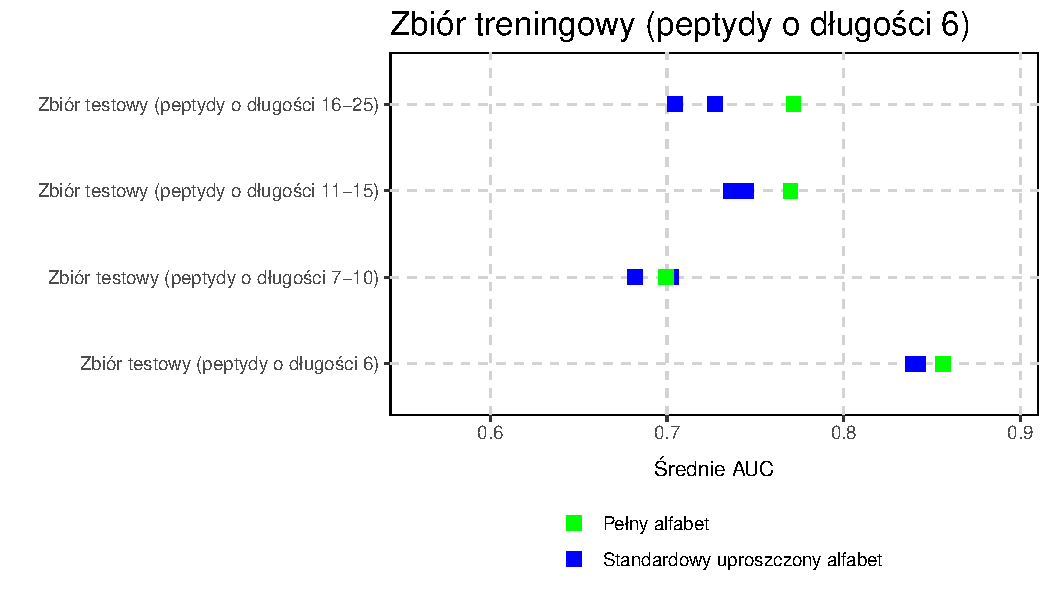
\includegraphics[width=\maxwidth]{figure/unnamed-chunk-6-1} 

Longer n-grams are more informative, but create larger feature spaces, which are hard to process and analyze.
\end{frame}

\begin{frame}{Permutation Tests}
  Informative n-grams are usually selected using permutation tests.

During a permutation test we shuffle randomly class labels and compute a defined statistic (e.g. information gain). Values of statistic for permuted data are compared with the value of statistic for original data.

$$
\textrm{p-value} = \frac{N_{T_P > T_R}}{N} $$

$N_{T_P > T_R}$: number of cases, where $T_P$ (permuted test statistic) has more extreme values than $T_R$ (test statistic for original data).

$N$: number of permutations.
  \end{frame}

\begin{frame}{QuiPT}  


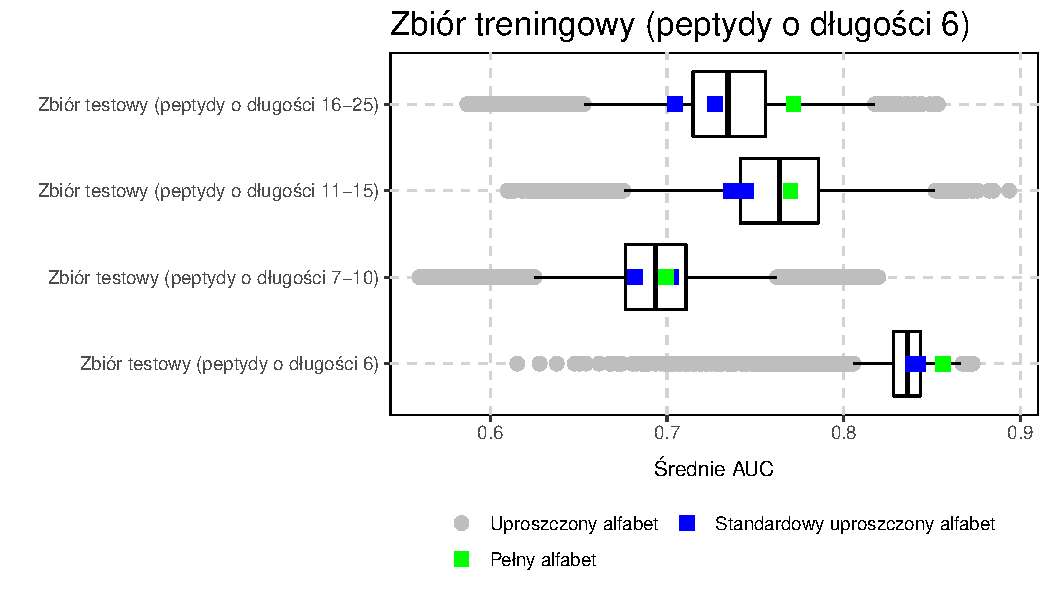
\includegraphics[width=\maxwidth]{figure/unnamed-chunk-7-1} 


QuiPT (available as part of the \textbf{biogram} R package) is faster than classical permutation tests and returns exact p-values.
\end{frame}

\section{Simplified alphabets}

\begin{frame}
Simplified alphabets:
\begin{itemize}
\item are based on grouping amino acids with similar physicochemical properties,
\item ease computational analysis of a sequence~\citep{murphy_simplified_2000},
\item create more explicite models.
\end{itemize}
\end{frame}


\begin{frame}  
Two sequences that are drastically different considering their amino acids composition can have the same physicochemical properties.




Sequence I: 

\texttt{FKVWPDHGSG}

\medskip

Sequence II: 

\texttt{YMCIYRAQTN}

\end{frame}  


\begin{frame}

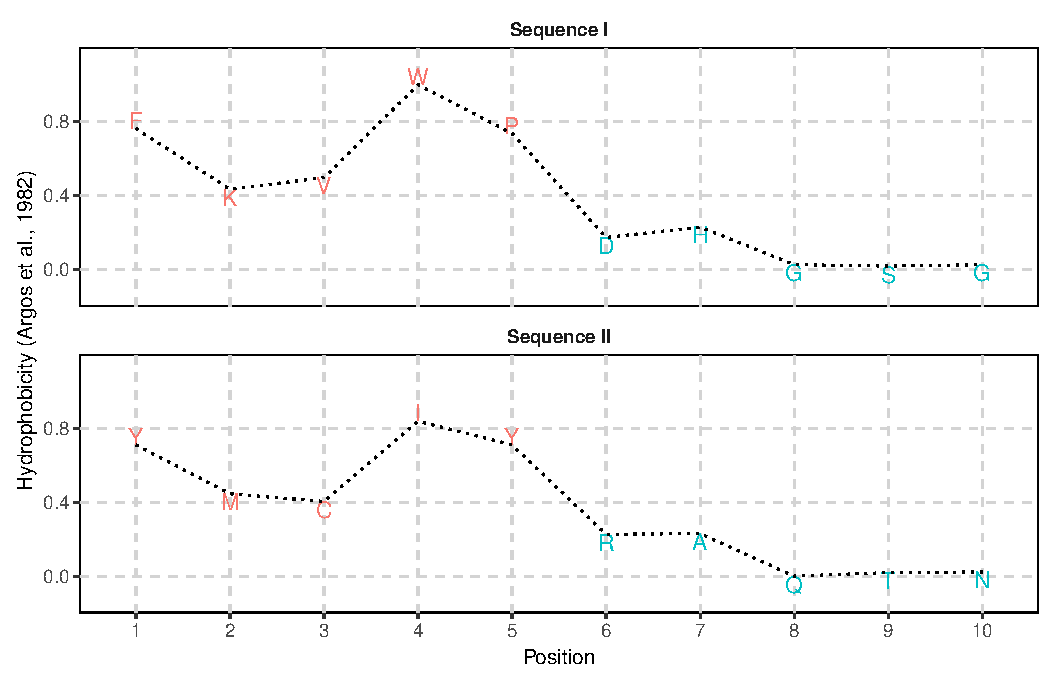
\includegraphics[width=\maxwidth]{figure/unnamed-chunk-9-1} 


\end{frame}  

\begin{frame}
\begin{table}
\begin{tabular}{cl}
\toprule
Subgroup & Amino acid \\ 
\midrule
  1 & C, I, L, K, M, F, P, W, Y, V \\ 
\rowcolor[gray]{0.85}  2 & A, D, E, G, H, N, Q, R, S, T \\ 
\bottomrule
\end{tabular}
\end{table}

\begin{columns}
\begin{column}{0.44\textwidth}
 
Sequence I: \texttt{FKVWPDHGSG} \textrightarrow

Sequence II: \texttt{YMCIYRAQTN} \textrightarrow

\end{column}
\begin{column}{0.5\textwidth}  %%<--- here

\texttt{1111122222}

\texttt{1111122222}
\end{column}
\end{columns}
\end{frame}  



\section{Prediction of amyloidogenicity}

\begin{frame}{AmyloGram}
AmyloGram: n-gram based tool for prediction of amyloid proteins~\citep{burdukiewicz_prediction_2016}.
\end{frame}


    \begin{frame}
\begin{figure} 
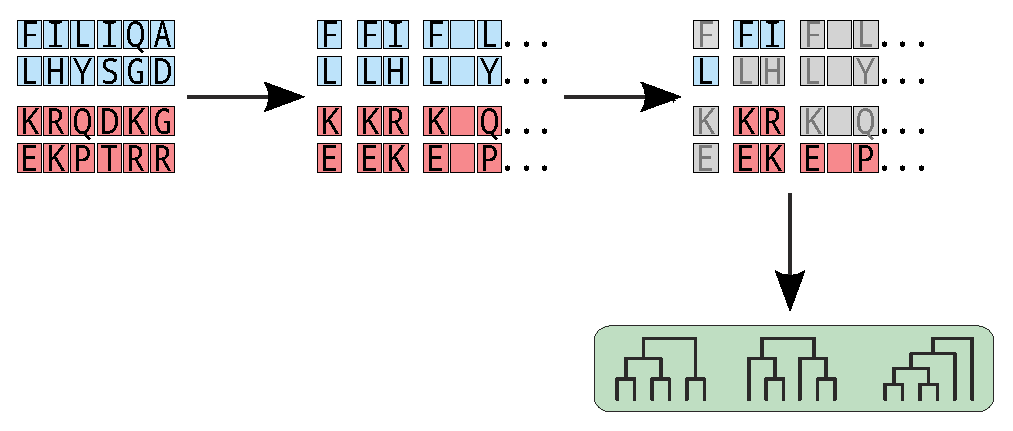
\includegraphics[width=0.95\textwidth]{static_figure/ngram1.eps}
\end{figure}
  \end{frame}

\begin{frame}{Cross-validation}
\begin{knitrout}
\definecolor{shadecolor}{rgb}{0.969, 0.969, 0.969}\color{fgcolor}

{\centering 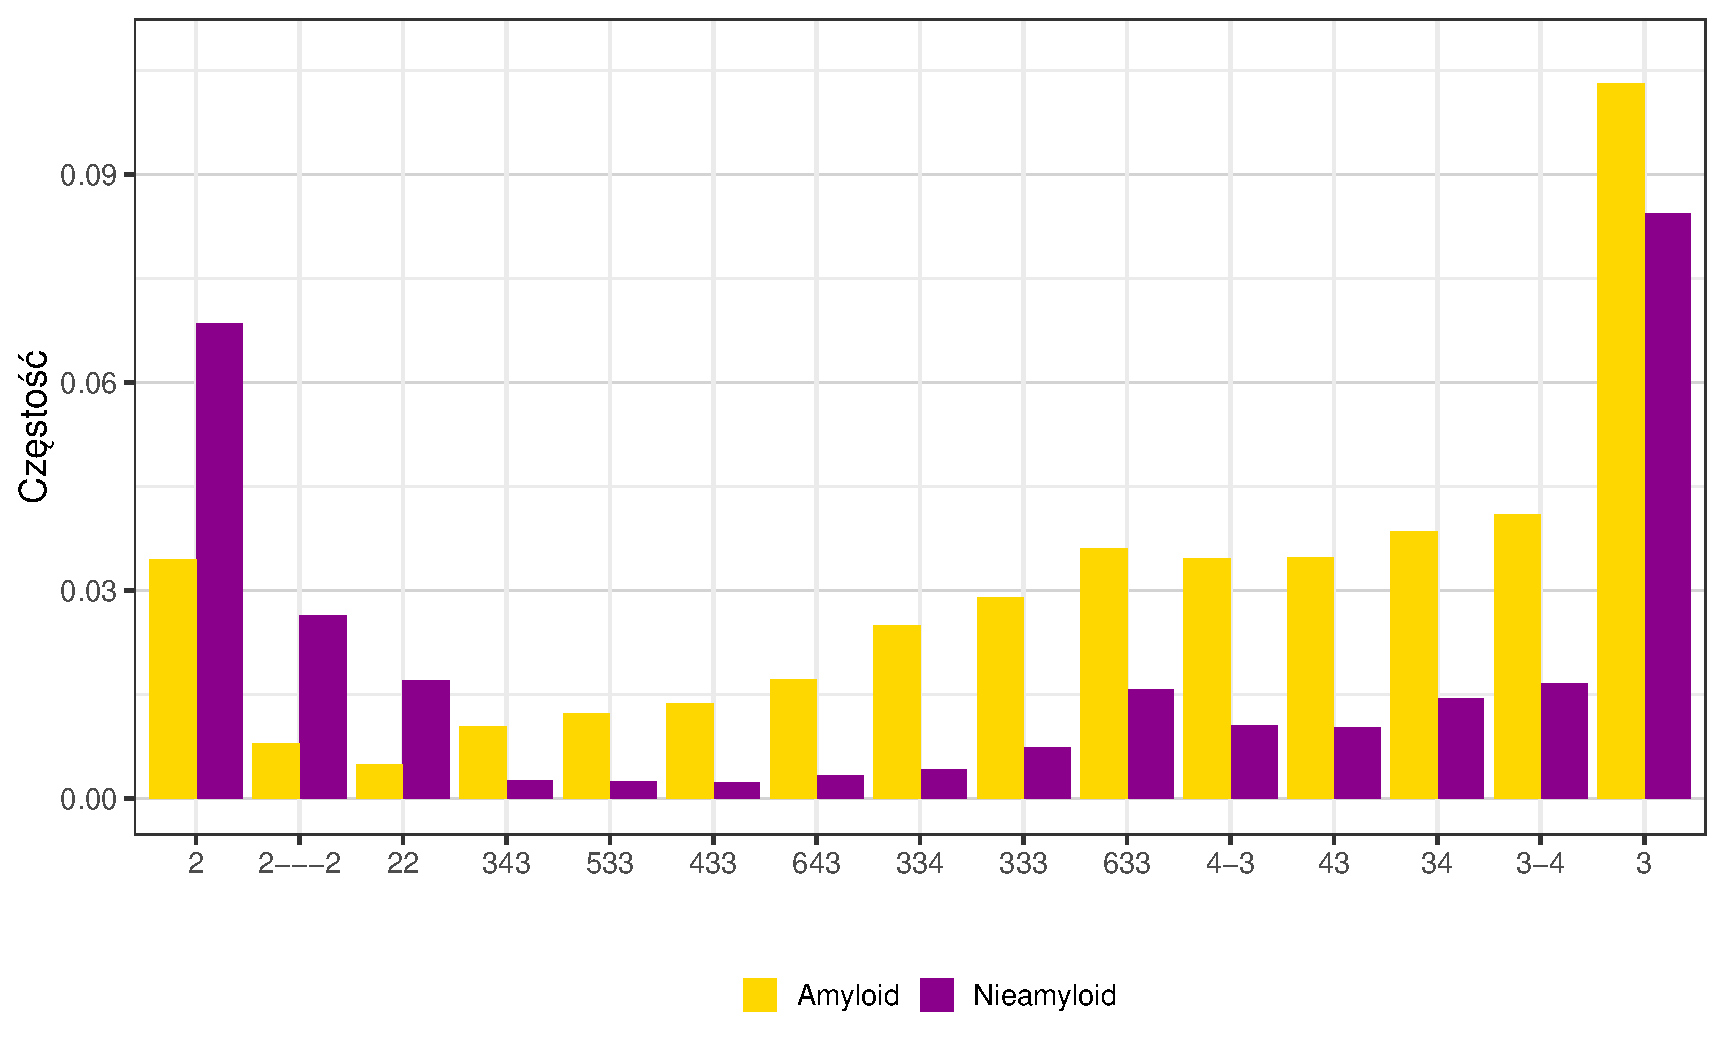
\includegraphics[width=\maxwidth]{figure/unnamed-chunk-10-1} 

}



\end{knitrout}
AUC (Area Under the Curve) measures the performance of a classifier (1 - classifier always properly recognizes amyloid proteins, 0 - classifier never properly recognizes amyloid proteins).

\end{frame}


\begin{frame}
  Does amyloidogenicity depend on the exact sequence of amino acids?
  \end{frame}

\begin{frame}{Standard simplified amino acid alphabets}
To date, several simplified amino acid alphabets have been proposed, which have been applied to (among others) protein folding and protein structure prediction~\citep{kosiol_new_2004, melo_accuracy_2006}.
  \end{frame}
  
    \begin{frame}{Standard simplified amino acid alphabets}
\begin{figure} 
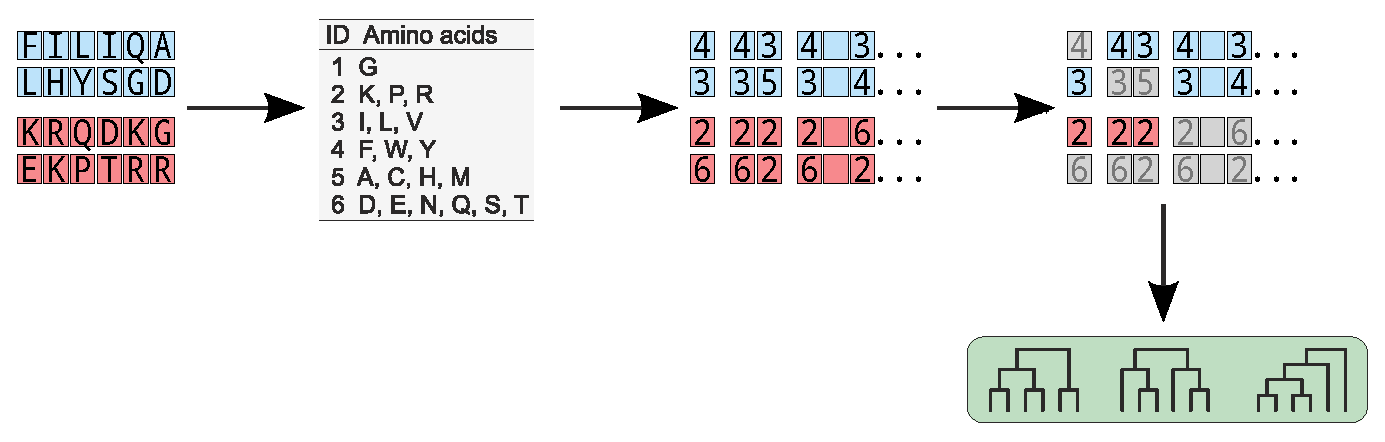
\includegraphics[width=0.95\textwidth]{static_figure/ngram2.eps}
\end{figure}


  \end{frame}


    \begin{frame}{Cross-validation}
\begin{knitrout}
\definecolor{shadecolor}{rgb}{0.969, 0.969, 0.969}\color{fgcolor}

{\centering 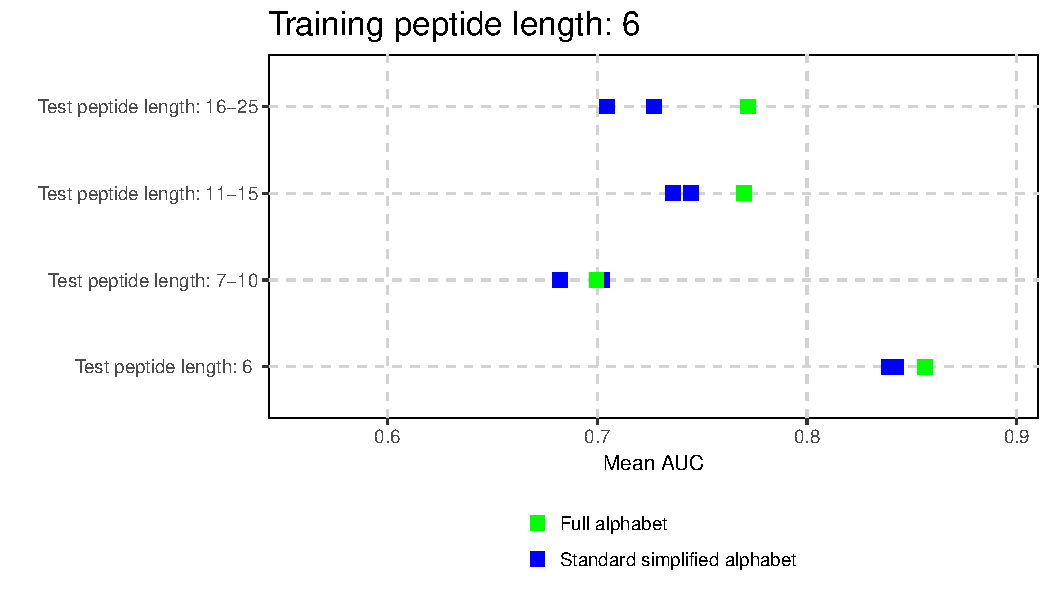
\includegraphics[width=\maxwidth]{figure/unnamed-chunk-11-1} 

}



\end{knitrout}

Standard simplified amino acid alphabets do not enhance discrimination between amyloidogenic and non-amyloidogenic proteins.
  
  \end{frame}


\begin{frame}{Novel simplified amino acid alphabets}

\begin{itemize}
\item 17 measures handpicked from AAIndex database: 
  \begin{itemize}
    \item size of residues, 
    \item hydrophobicity, 
    \item solvent surface area, 
    \item frequency in $\beta$-sheets,
    \item contactivity.
  \end{itemize}
  \item 524 284 amino acid simplified alphabets with different level of amino acid alphabet reduction (three to six amino acid groups).
  \end{itemize}

    \end{frame}
  
    \begin{frame}{Novel simplified amino acid alphabets}
\begin{figure} 
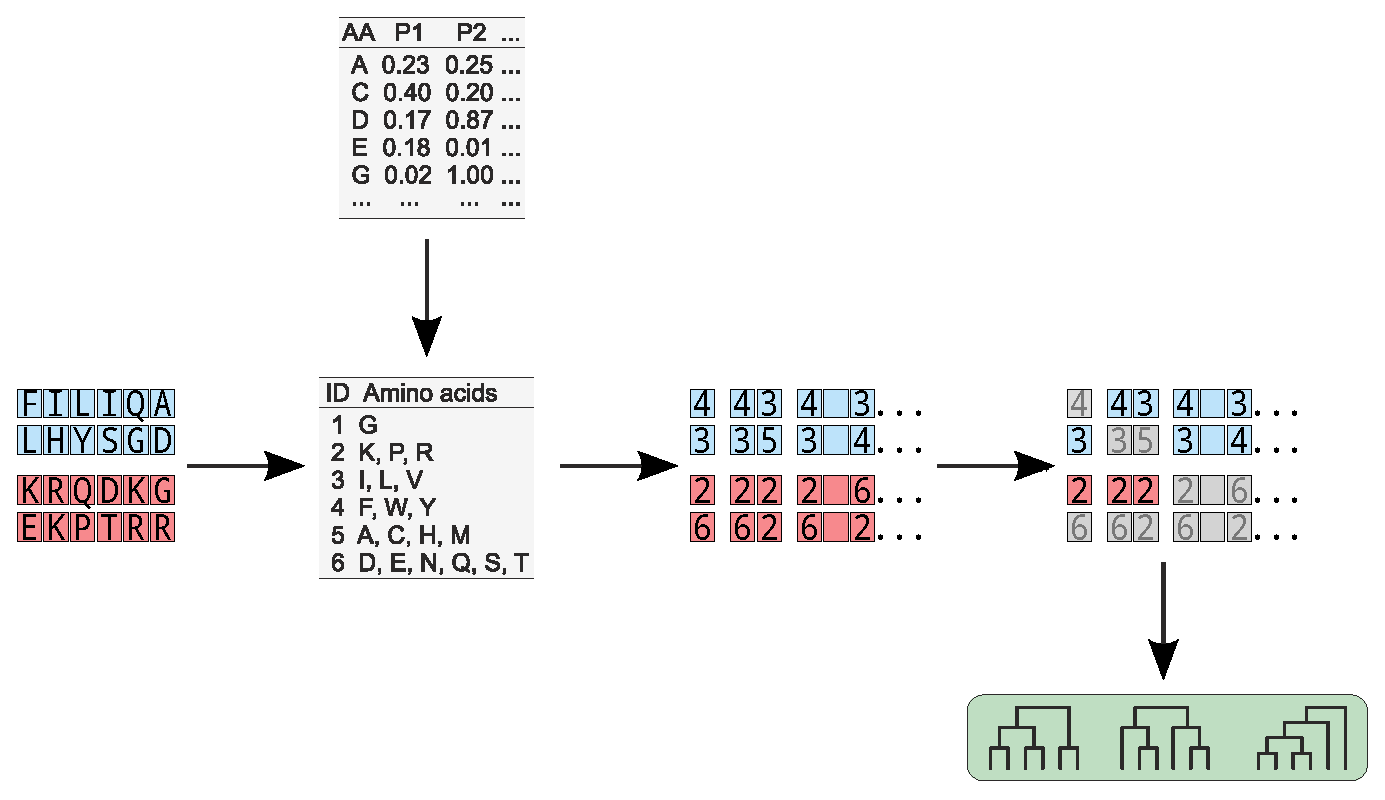
\includegraphics[width=0.95\textwidth]{static_figure/ngram3.eps}
\end{figure}
  \end{frame}



\begin{frame}{Cross-validation}
\begin{knitrout}
\definecolor{shadecolor}{rgb}{0.969, 0.969, 0.969}\color{fgcolor}

{\centering 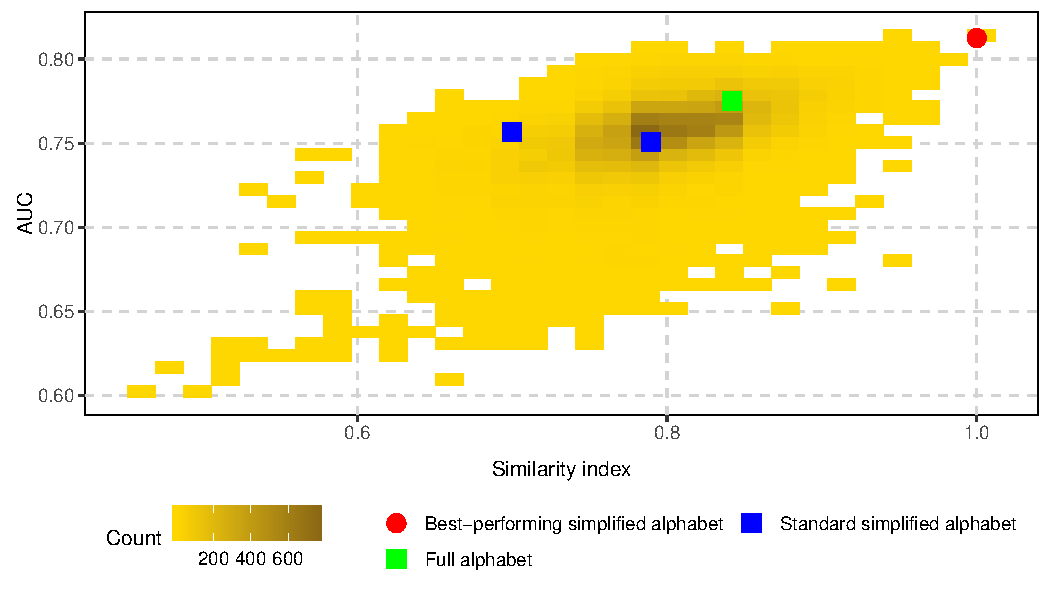
\includegraphics[width=\maxwidth]{figure/unnamed-chunk-12-1} 

}



\end{knitrout}
  \small
Hinges of boxes correspond to 
the 0.25 and 0.75 quartiles. The bar inside the box represents the median. The 
gray circles correspond to the simplified alphabets with the AUC outside the 0.95 
confidence interval.

  
  \end{frame}


  
    \begin{frame}{The best-performing simplified alphabet}
\begin{knitrout}
\definecolor{shadecolor}{rgb}{0.969, 0.969, 0.969}\color{fgcolor}

{\centering 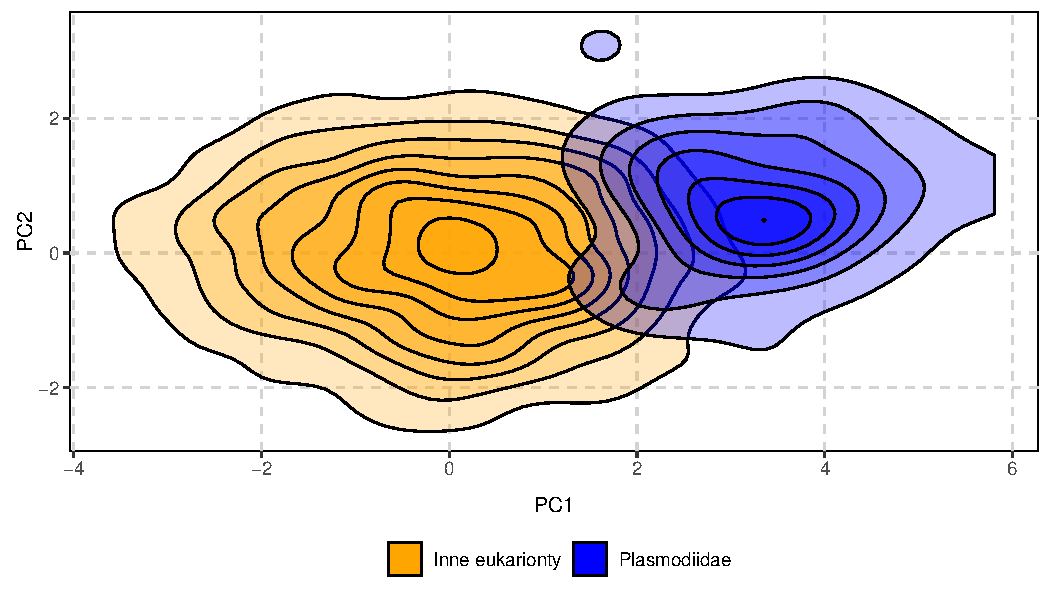
\includegraphics[width=\maxwidth]{figure/unnamed-chunk-13-1} 

}



\end{knitrout}
  \end{frame}

     \begin{frame}{The best-performing simplified alphabet}

   \begin{table}[ht]
\centering
\begin{tabular}{rl}
  \toprule
Subgroup ID & Amino acids \\ 
  \midrule
  1 & G \\ 
   \rowcolor[gray]{0.85}  2 & K, P, R \\ 
    3 & I, L, V \\ 
   \rowcolor[gray]{0.85}  4 & F, W, Y \\ 
    5 & A, C, H, M \\ 
   \rowcolor[gray]{0.85}  6 & D, E, N, Q, S, T \\ 
   \bottomrule
\end{tabular}
\end{table}
   
   \end{frame}

     \begin{frame}{The best-performing simplified alphabet}
   \begin{table}[ht]
\centering
\begin{tabular}{rl}
  \toprule
Subgroup ID & Amino acids \\ 
  \midrule
  1 & G \\ 
   \rowcolor[gray]{0.85}  2 & K, P, R \\ 
   \rowcolor{blue!20} 3 & I, L, V \\ 
   \rowcolor{blue!20}  4 & F, W, Y \\ 
    5 & A, C, H, M \\ 
   \rowcolor[gray]{0.85}  6 & D, E, N, Q, S, T \\ 
   \bottomrule
\end{tabular}
\end{table}
   
Group 3 and 4 - hydrophobic amino acids.  
   \end{frame}
  
  
     \begin{frame}{The best-performing simplified alphabet}
   \begin{table}[ht]
\centering
\begin{tabular}{rl}
  \toprule
Subgroup ID & Amino acids \\ 
  \midrule
  1 & G \\ 
   \rowcolor{red!20}  2 & K, P, R \\ 
    3 & I, L, V \\ 
   \rowcolor[gray]{0.85}  4 & F, W, Y \\ 
    5 & A, C, H, M \\ 
   \rowcolor[gray]{0.85}  6 & D, E, N, Q, S, T \\ 
   \bottomrule
\end{tabular}
\end{table}
   
Group 2 - charged breakers of $\beta$-structures.  
   
   \end{frame}  
   
\begin{frame}{Alphabet similarity and performance}
Is the best-performing simplified amino alphabet associated with amyloidogenicity?
\end{frame}

\begin{frame}{Similarity index}
\begin{knitrout}
\definecolor{shadecolor}{rgb}{0.969, 0.969, 0.969}\color{fgcolor}

{\centering 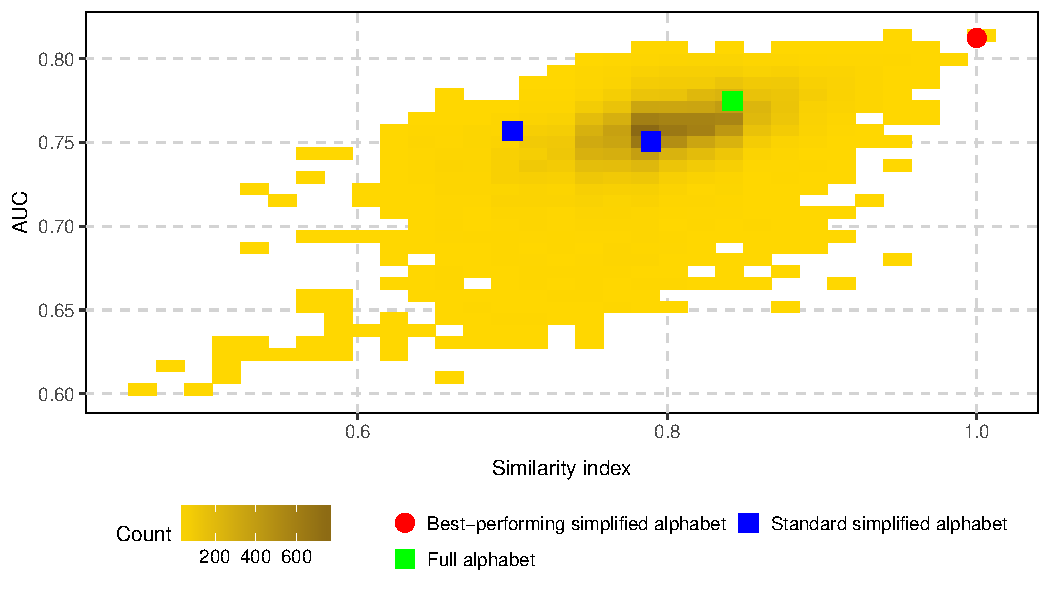
\includegraphics[width=\maxwidth]{figure/unnamed-chunk-15-1} 

}



\end{knitrout}
Similarity index~\citep{stephenson_unearthing_2013} measures the similarity between two simplified alphabets (1 - identical, 0, totally dissimilar).
\end{frame}



\begin{frame}{Similarity index}
\begin{knitrout}
\definecolor{shadecolor}{rgb}{0.969, 0.969, 0.969}\color{fgcolor}

{\centering 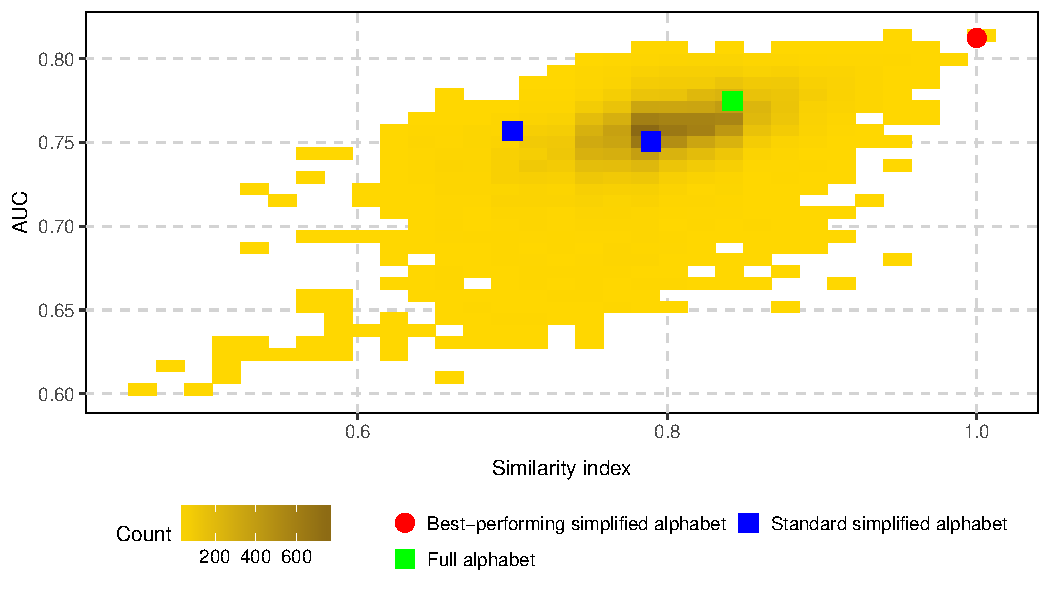
\includegraphics[width=\maxwidth]{figure/unnamed-chunk-16-1} 

}



\end{knitrout}
The color of a square is proportional to the number of simplified alphabets in its area.
\end{frame}

\begin{frame}{Similarity index}
\begin{knitrout}
\definecolor{shadecolor}{rgb}{0.969, 0.969, 0.969}\color{fgcolor}

{\centering 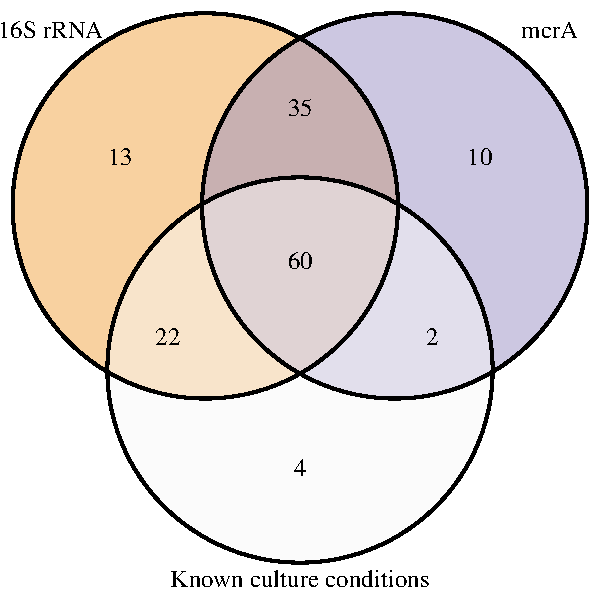
\includegraphics[width=\maxwidth]{figure/unnamed-chunk-17-1} 

}



\end{knitrout}
The correlation between mean AUC an similarity index is significant ($\textrm{p-value} \leq 2.2^{-16}$; $\rho = 0.51$).
\end{frame}
   
\begin{frame}{}
Are informative n-grams found by QuiPT associated with amyloidogenicity?
\end{frame}


\begin{frame}{Informative n-grams}
\begin{knitrout}
\definecolor{shadecolor}{rgb}{0.969, 0.969, 0.969}\color{fgcolor}

{\centering 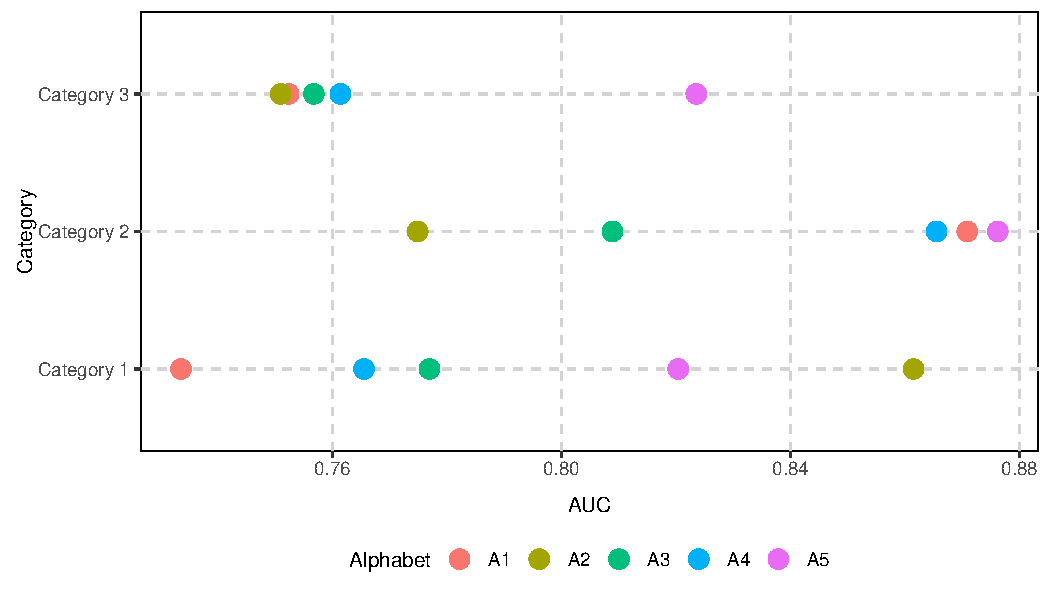
\includegraphics[width=\maxwidth]{figure/unnamed-chunk-18-1} 

}



\end{knitrout}

Out of 65 the most informative n-grams, 15 (23\%) were also found in the motifs validated experimentally~\citep{paz_sequence_2004}.
\end{frame}


\begin{frame}{Benchmark results}

\begin{table}[ht]
\centering

\begin{tabular}{ccccc}
  \toprule
Classifier & AUC & MCC \\ 
  \midrule
AmyloGram & \textbf{0.8972} & \textbf{0.6307} \\ 
  \rowcolor{white}PASTA 2.0 \citep{walsh_pasta_2014} & 0.8550 & 0.4291  \\ 
   FoldAmyloid \citep{garbuzynskiy_foldamyloid:_2010} & 0.7351 & 0.4526  \\ 
  \rowcolor{white}APPNN \citep{familia_prediction_2015} & 0.8343 & 0.5823  \\ 
   \bottomrule
\end{tabular}
\end{table}

The predictor based on the best-performing alphabet, called AmyloGram, was benchmarked against the most popular tools for the detection of amyloid peptides using an external data set \textit{pep424}.

\footnotesize

\end{frame}

\begin{frame}{Benchmark results}

\begin{table}[ht]
\centering

\begin{tabular}{ccccc}
  \toprule
Classifier & AUC & MCC \\ 
  \midrule
AmyloGram & \textbf{0.8972} & \textbf{0.6307} \\ 
  \rowcolor{white}PASTA 2.0 \citep{walsh_pasta_2014} & 0.8550 & 0.4291  \\ 
   FoldAmyloid \citep{garbuzynskiy_foldamyloid:_2010} & 0.7351 & 0.4526  \\ 
  \rowcolor{white}APPNN \citep{familia_prediction_2015} & 0.8343 & 0.5823  \\ 
   \bottomrule
\end{tabular}
\end{table}

MCC (Matthew's Correlation Coefficient) measures the performance of a classifier (1 - classifier always properly recognizes amyloid proteins, -1 - classifier never properly recognizes amyloid proteins).

\footnotesize

\end{frame}



\begin{frame}{Experimental validation}
\begin{figure} 
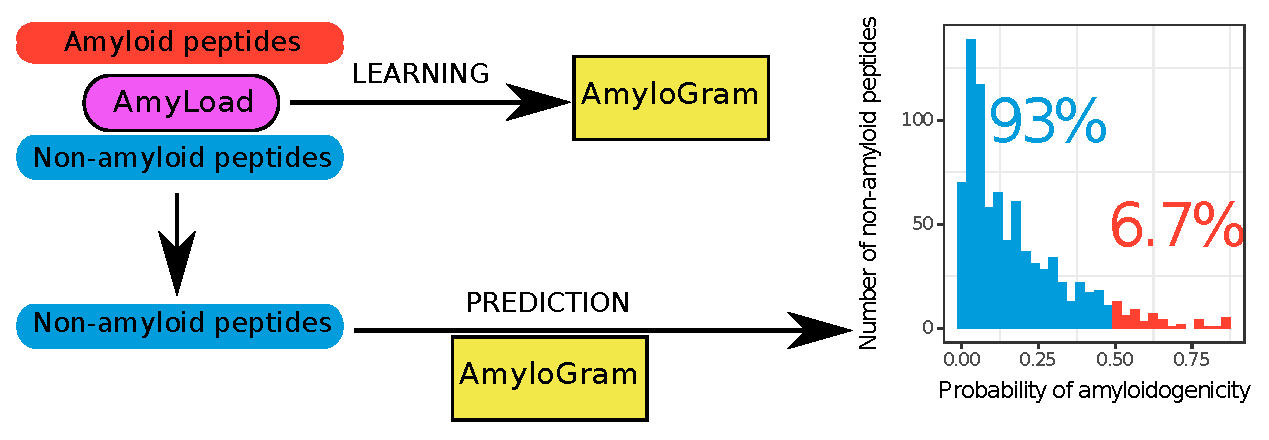
\includegraphics[width=0.95\textwidth]{static_figure/diagram1.eps}
\end{figure}
\end{frame}

\begin{frame}{Experimental validation}
\begin{figure} 
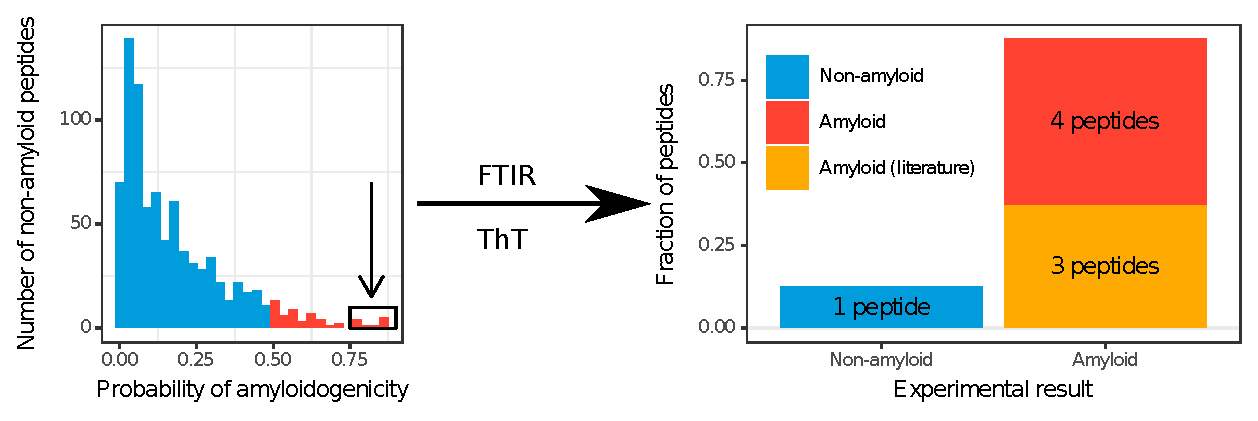
\includegraphics[width=0.95\textwidth]{static_figure/diagram2.eps}
\end{figure}
\end{frame}

\section{Other applications}

\begin{frame}{Signal peptide prediction}

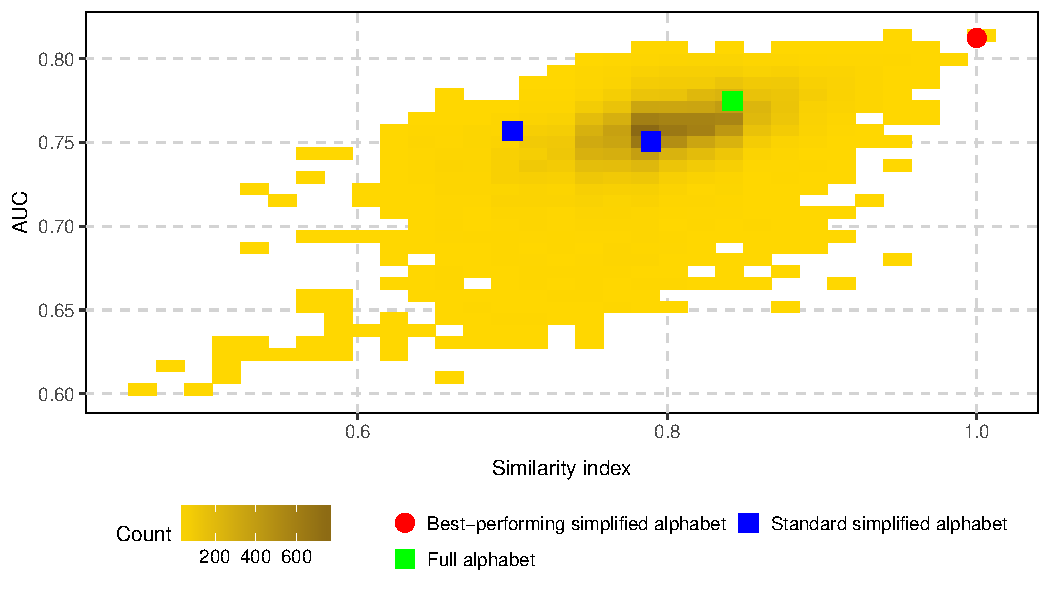
\includegraphics[width=\maxwidth]{figure/unnamed-chunk-19-1} 

PCA of amino acid frequency in signal peptides.

\end{frame}  


\begin{frame}{Signal peptide prediction}
\begin{figure} 
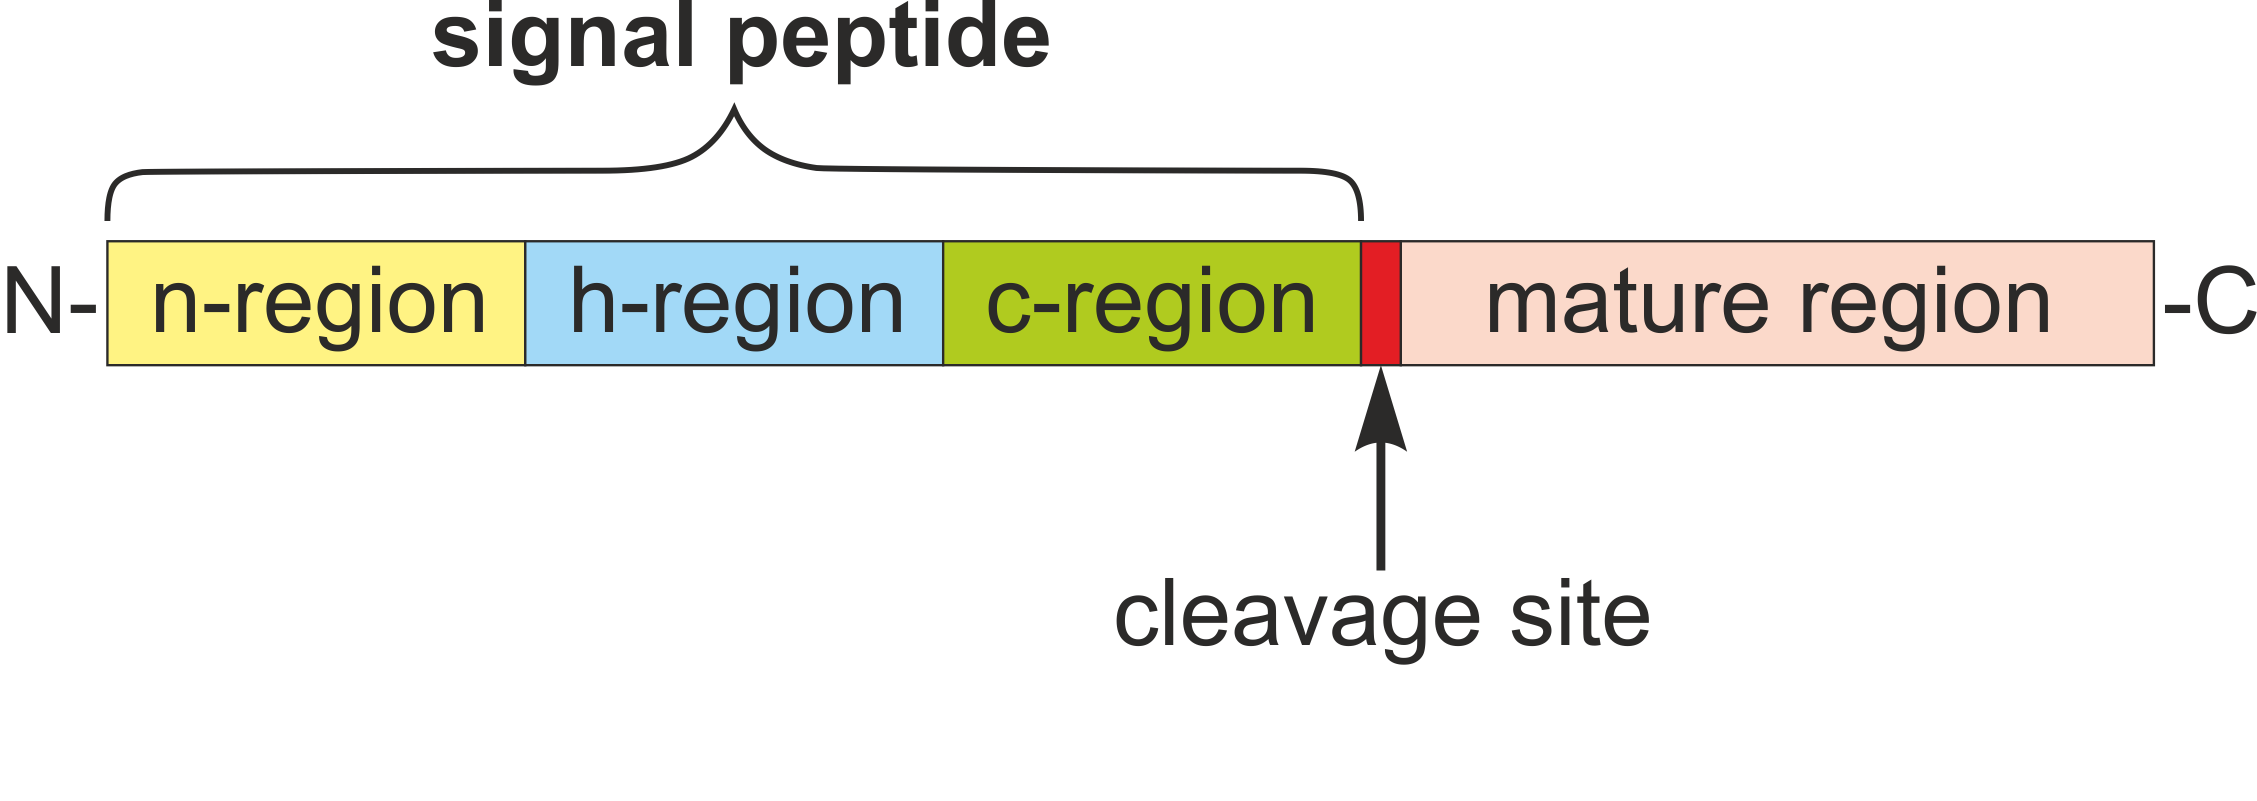
\includegraphics[width=0.75\textwidth]{static_figure/SP.png}
\end{figure}
SignalP 4.1~\citep{petersen_signalp_2011} combines output of two separate predictors:
\begin{itemize}
\item cleavage site,
\item signal peptide.
\end{itemize}
\end{frame}

\begin{frame}{Signal peptide prediction}

\begin{knitrout}
\definecolor{shadecolor}{rgb}{0.969, 0.969, 0.969}\color{fgcolor}

{\centering 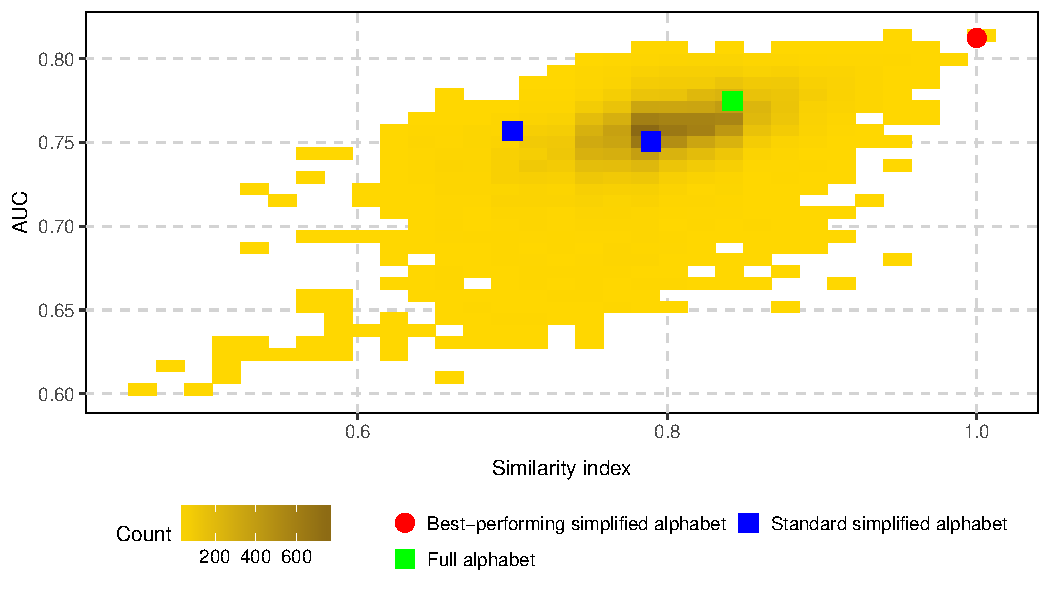
\includegraphics[width=\maxwidth]{figure/unnamed-chunk-20-1} 

}



\end{knitrout}
\end{frame}

\begin{frame}{Prediction of culturing conditions}
\begin{knitrout}
\definecolor{shadecolor}{rgb}{0.969, 0.969, 0.969}\color{fgcolor}

{\centering 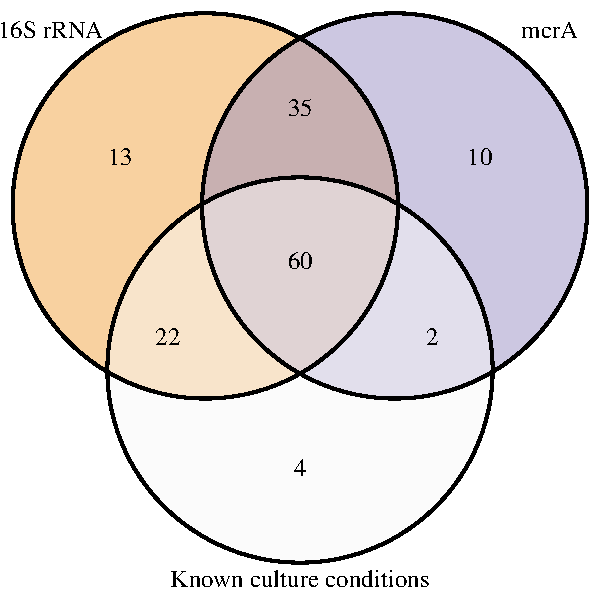
\includegraphics[width=170,height=150]{figure/unnamed-chunk-21-1} 

}



\end{knitrout}
\url{metanogen.biotech.uni.wroc.pl}~\citep{jablonski2015methanogenic}

\end{frame}

\begin{frame}{Prediction of culturing conditions}
Results of nested cross-validation of MethanoGram.
\begin{table}[ht]
\centering
\begin{tabular}{ll}
  \hline
Culturing condition & Mean error \\ 
  \hline
Growth rate [h$^{-1}$] & 0.35 \\ 
Growth doubling time [h] &  27.19 \\ 
Optimal growth temp. [$^{\circ}$C] & 8.89 \\ 
Optimal growth pH & 0.47 \\ 
Optimal growth NaCl [mol/dm$^3$] & 0.21 \\ 
   \hline
\end{tabular}
\label{tab:nested_cv}
\end{table}

\end{frame}  



\begin{frame}{Summary}
\begin{enumerate}
\item Created algorithms effectively filtering n-grams.

\item Introduced new methods for search of simplified amino acids.

\item Implemented novel algorithms in the \textbf{R} package \textit{biogram}.

\item Applied the n-gram analysis framework to:
\begin{itemize}
\item prediction of amyloids (AmyloGram) (to appear in Scientific Reports),
\item prediction of atypical signal peptides,
\item prediction of culture conditions of methanogenes (MethanoGram).
\end{itemize}
\end{enumerate}
\end{frame}  

\begin{frame}{Summary}

Web servers:
\begin{itemize}
\item \textbf{AmyloGram}: \url{http://www.smorfland.uni.wroc.pl/shiny/AmyloGram/}.
\item \textbf{MethanoGram}: \url{http://www.smorfland.uni.wroc.pl/shiny/MethanoGram/}.
\item \textbf{signalHsmm}: \url{http://www.smorfland.uni.wroc.pl/shiny/signalHsmm/}.
\end{itemize}


Software packages:
\begin{itemize}
\item \textbf{biogram}: \url{https://cran.r-project.org/package=biogram}.
\item \textbf{AmyloGram}: \url{https://cran.r-project.org/package=AmyloGram}.
\end{itemize}


\end{frame}  

\begin{frame}{Acknowledgments}
Mentors:
\begin{itemize}
\item \textbf{Paweł Mackiewicz (University of Wrocław)}.
\item Lars Kaderali (University of Greifswald).
\item Małgorzata Kotulska (Wrocław University of Science and Technology).
\item Marcin Łukaszewicz (University of Wrocław).
\item Henrik Nielsen (Technical University of Denmark).
\item Stefan Rödiger (Brandenburg University of Technology Cottbus-Senftenberg).
\item Andreas Weinhäusel (Austrian Institute of Technology).
\end{itemize}
\end{frame}


\begin{frame}{Acknowledgments}
Peers:
\begin{itemize}
\item Agata Błaszczyńska (Wrocław University of Science and Technology).
\item Anna Duda-Madej (Wrocław Medical University).
\item Przemysław Gagat (University of Wrocław).
\item Marlena G\k{a}sior-Głogowska (Wrocław University of Science and Technology).
\item Sławomir Jabłoński (University of Wrocław).
\item Rafał Kolenda (Sanger Institute).
\item Chris Lauber (Technical University Dresden).
\item Natalia Niedzielska (Wrocław University of Science and Technology).
\item Piotr Sobczyk (Wrocław University of Science and Technology).
\end{itemize}

\end{frame}

\begin{frame}{Acknowledgments}
Funding:
\begin{itemize}
\item National Science Center (Preludium and Etiuda).
\item COST ACTION CA15110 (Harmonising standardisation strategies to increase efficiency and competitiveness of European life-science research).
\item KNOW Wrocław Center for Biotechnology.
\end{itemize}

\end{frame}

\begin{frame}[allowframebreaks]{Publications}

\small
\begin{enumerate}
\item \textbf{Burdukiewicz, M.}, Sobczyk, P., Rödiger, S., Duda-Madej, A., Mackiewicz, P., and Kotulska, M. (2017). Amyloidogenic motifs revealed by n-gram analysis. Scientific Reports (accepted).

\item Rödiger, S., \textbf{Burdukiewicz, M.}, Spiess, A.-N., and Blagodatskikh, K. (2017). Enabling reproducible real-time quantitative PCR research: the RDML package. Bioinformatics.

\item Schiebel, J., Böhm, A., Nitschke, J., \textbf{Burdukiewicz, M.}, Weinreich, J., Ali, A., Roggenbuck, D., Rödiger, S., and Schierack, P. (2017). Genotypic and phenotypic characteristics in association with biofilm formation in different pathotypes of human clinical Escherichia coli isolates. Appl. Environ. Microbiol. AEM.01660-17.

\item \textbf{Burdukiewicz, M.}, Rödiger, S., Sobczyk, P., Menschikowski, M., Schierack, P., and Mackiewicz, P. (2016a). Methods for comparing multiple digital PCR experiments. Biomolecular Detection and Quantification 9, 14–19.

\item \textbf{Burdukiewicz, M.}, Sobczyk, P., Rödiger, S., Duda-Madej, A., Mackiewicz, P., and Kotulska, M. (2016b). Prediction of amyloidogenicity based on the n-gram analysis. PeerJ Preprints.

\item Spiess, A.-N., Rödiger, S., \textbf{Burdukiewicz, M.}, Volksdorf, T., and Tellinghuisen, J. (2016). System-specific periodicity in quantitative real-time polymerase chain reaction data questions threshold-based quantitation. Scientific Reports.

\item Rödiger, S., \textbf{Burdukiewicz, M.}, Blagodatskikh, K., Jahn M., and Schierack, P. (2016). R as an Environment for Reproducible Analysis of DNA Amplification Experiments (R Journal).

\item Rödiger, S., \textbf{Burdukiewicz, M.}, and Schierack, P. (2015). chipPCR: an R package to pre-process raw data of amplification curves. Bioinformatics 31, 2900–2902.

\item Spiess, A.-N., Deutschmann, C., \textbf{Burdukiewicz, M.}, Himmelreich, R., Klat, K., Schierack, P., and Rödiger, S. (2015). Impact of Smoothing on Parameter Estimation in Quantitative DNA Amplification Experiments. Clinical Chemistry 61, 379–388.

\item Kolenda, R., \textbf{Burdukiewicz, M.}, and Schierack, P. (2015). A systematic review and meta-analysis of the epidemiology of pathogenic Escherichia coli of calves and the role of calves as reservoirs for human pathogenic E. coli. Frontiers in Cellular and Infection Microbiology 5.
\end{enumerate}

\end{frame}

\begin{frame}{Summary}
\begin{enumerate}
\item Created a new algorithm for effective filtering of n-grams.

\item Introduced new methods for search of simplified amino acids.

\item Implemented novel algorithms in the \textbf{R} package \textit{AmyloGram}.

\item Applied the n-gram analysis framework to:
\begin{itemize}
\item prediction of amyloids (AmyloGram),
\item prediction of atypical signal peptides,
\item prediction of culture conditions of methanogenes (MethanoGram).
\end{itemize}
\end{enumerate}
\end{frame}  


\begin{frame}[allowframebreaks]
        \frametitle{References}
  \bibliographystyle{apalike}
  \bibliography{references}
\end{frame}  

\begin{frame}{Ranking alphabets}
\begin{knitrout}
\definecolor{shadecolor}{rgb}{0.969, 0.969, 0.969}\color{fgcolor}

{\centering 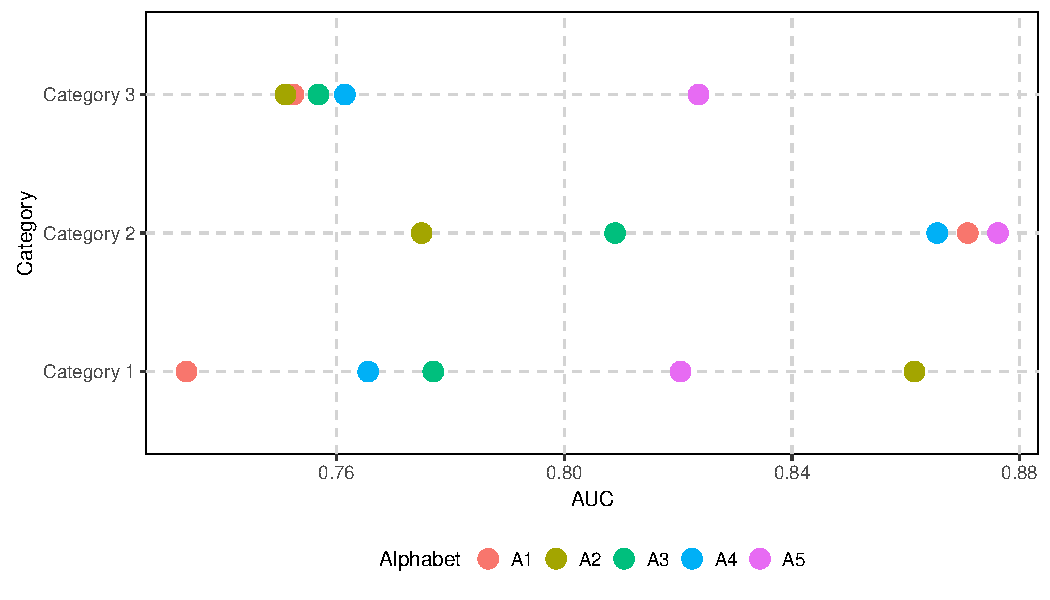
\includegraphics[width=\maxwidth]{figure/unnamed-chunk-22-1} 

}



\end{knitrout}
\end{frame}


\begin{frame}{Ranking alphabets}
\begin{knitrout}
\definecolor{shadecolor}{rgb}{0.969, 0.969, 0.969}\color{fgcolor}

{\centering 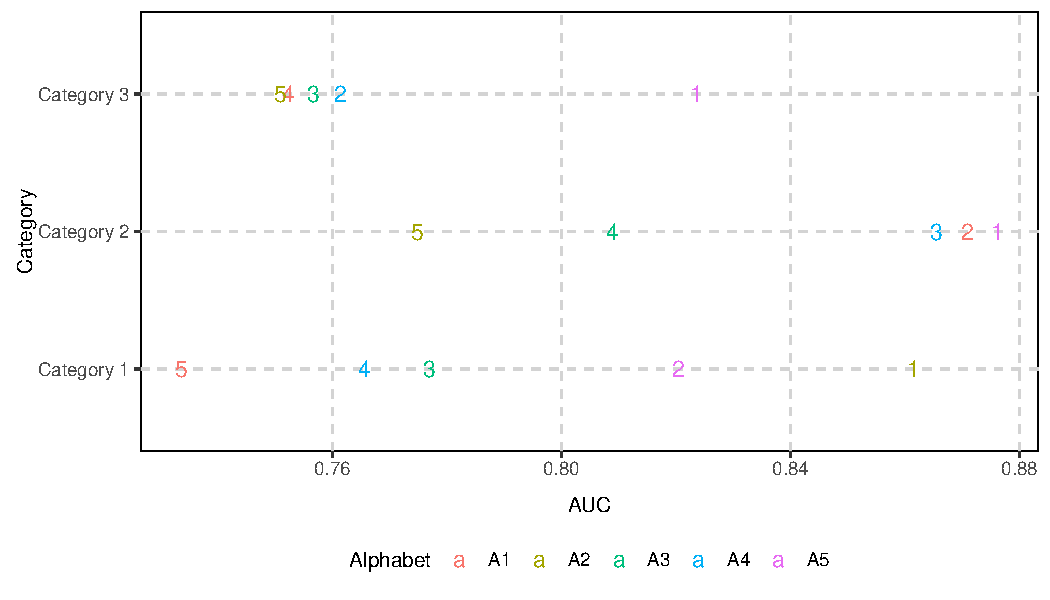
\includegraphics[width=\maxwidth]{figure/unnamed-chunk-23-1} 

}



\end{knitrout}
We rank alphabets separately in all length categories assuming the rank 1 for the best AUC, rank 2 for the second best AUC and so on.


\end{frame}



\begin{frame}{Ranking alphabets}
\begin{knitrout}
\definecolor{shadecolor}{rgb}{0.969, 0.969, 0.969}\color{fgcolor}

{\centering 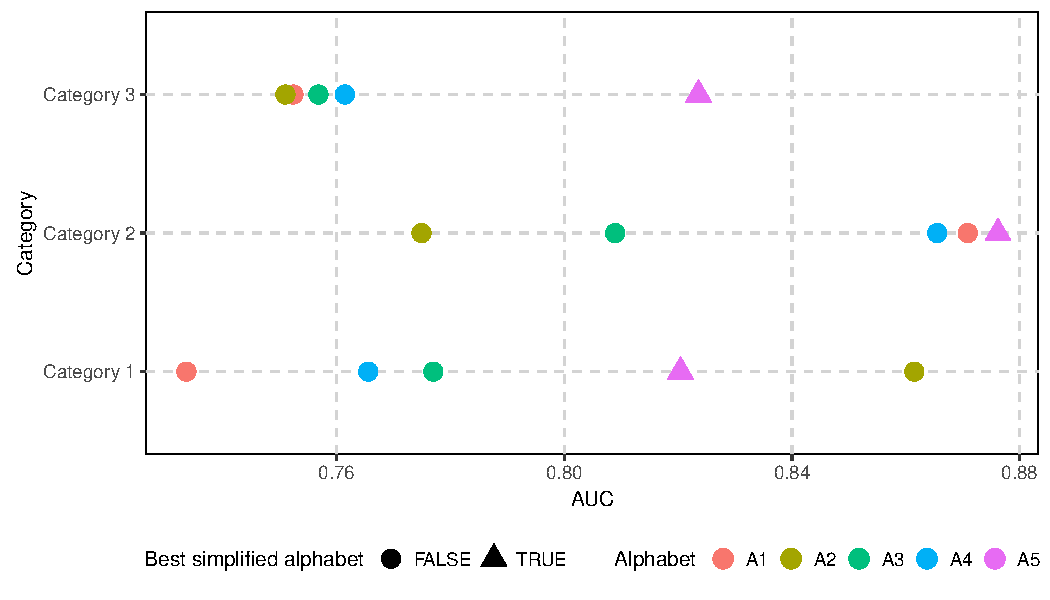
\includegraphics[width=\maxwidth]{figure/unnamed-chunk-24-1} 

}



\end{knitrout}
The best-performing alphabet has the lowest sum of ranks.  

\end{frame}


\end{document}
